\documentclass[16 pt]{amsart}
\usepackage{amscd,amsmath,amsthm,amssymb}
\usepackage{enumerate,varioref}
\usepackage{epsfig}
\usepackage{graphicx}
\usepackage{mathtools}
\usepackage{tikz}
\newtheorem{thm}{Theorem}
\newtheorem{cor}[thm]{Corollary}
\newtheorem{lem}[thm]{Lemma}
\newtheorem{prop}[thm]{Proposition}
\theoremstyle{definition}
\newtheorem{defn}[thm]{Definition}
\theoremstyle{remark}
\newtheorem{ex}[thm]{Example}
\newtheorem{rem}[thm]{Remark}
\numberwithin{equation}{subsection}
\newcommand{\R}{\mathbb{R}}
\newcommand{\Z}{\mathbb{Z}}
\newcommand{\C}{\mathbb{C}}
\newcommand{\Q}{\mathbb{Q}}
\newcommand{\lh}{\lim_{h\rightarrow 0}}
\begin{document}


\[
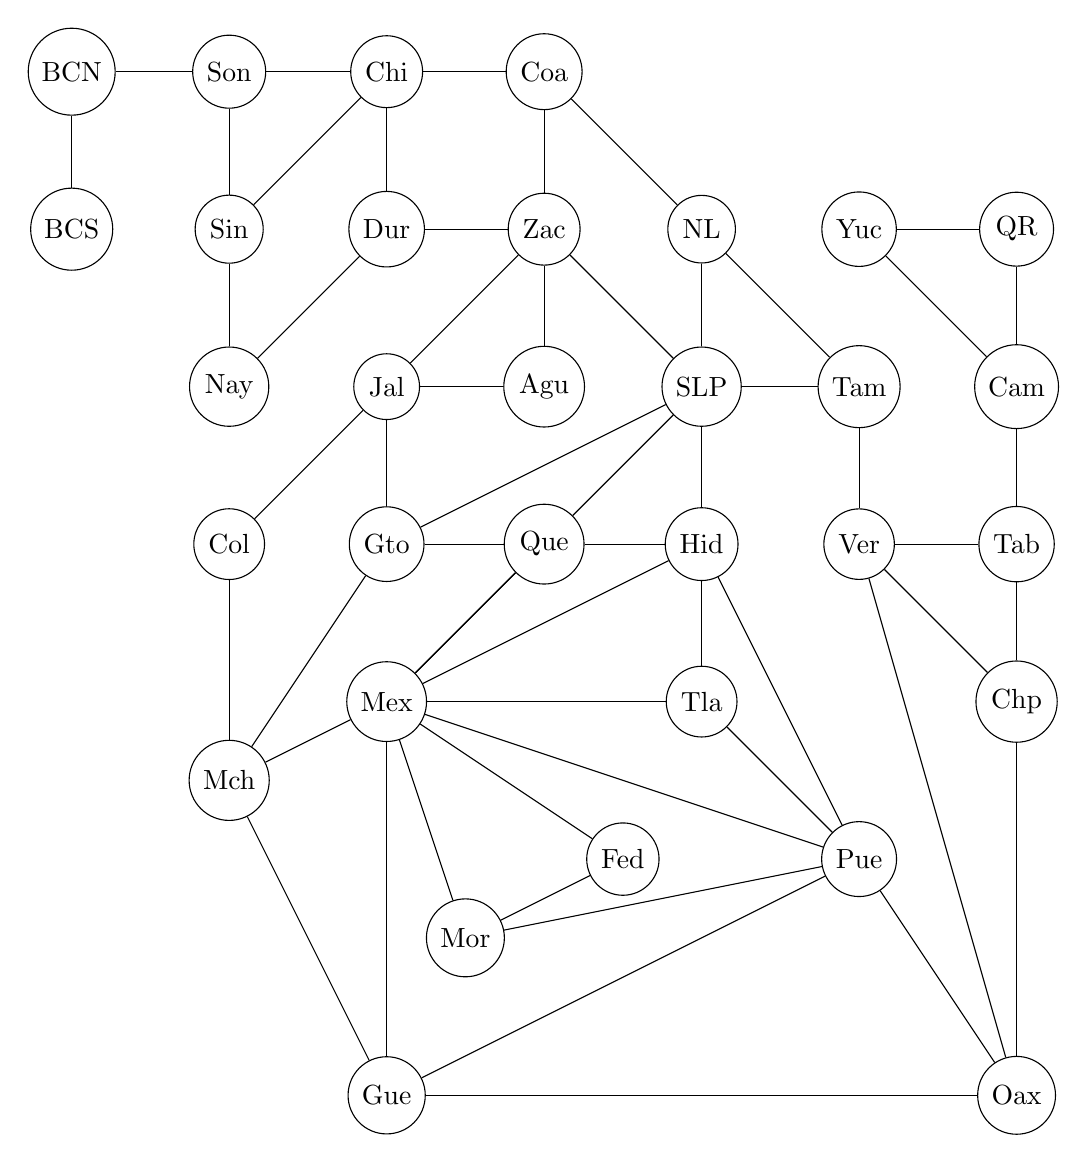
\begin{tikzpicture}
\node[circle,draw] (BCN) at (0,10){BCN};
\node[circle,draw] (BCS) at (0,8){BCS};
\node[circle,draw] (Son) at (2,10){Son};
\node[circle,draw] (Sin) at (2,8){Sin};
\node[circle,draw] (Nay) at (2,6){Nay};
\node[circle,draw] (Col) at (2,4){Col};
\node[circle,draw] (Mch) at (2,1){Mch};
\node[circle,draw] (Chi) at (4,10){Chi};
\node[circle,draw] (Dur) at (4,8){Dur};
\node[circle,draw] (Jal) at (4,6){Jal};
\node[circle,draw] (Gto) at (4,4){Gto};
\node[circle,draw] (Mex) at (4,2){Mex};
\node[circle,draw] (Gue) at (4,-3){Gue};
\node[circle,draw] (Coa) at (6,10){Coa};
\node[circle,draw] (Zac) at (6,8){Zac};
\node[circle,draw] (Agu) at (6,6){Agu};
\node[circle,draw] (Que) at (6,4){Que};
\node[circle,draw] (Fed) at (7,0){Fed};
\node[circle,draw] (Mor) at (5,-1){Mor};
\node[circle,draw] (NL) at (8,8){NL};
\node[circle,draw] (SLP) at (8,6){SLP};
\node[circle,draw] (Hid) at (8,4){Hid};
\node[circle,draw] (Tla) at (8,2){Tla};
\node[circle,draw] (Pue) at (10,0){Pue};
\node[circle,draw] (Oax) at (12,-3){Oax};
\node[circle,draw] (Tam) at (10,6){Tam};
\node[circle,draw] (Ver) at (10,4){Ver};
\node[circle,draw] (Tab) at (12,4){Tab};
\node[circle,draw] (Chp) at (12,2){Chp};
\node[circle,draw] (Cam) at (12,6){Cam};
\node[circle,draw] (Yuc) at (10,8){Yuc};
\node[circle,draw] (QR) at (12,8){QR};
\foreach \from/\to in {BCS/BCN,BCN/Son,Son/Sin,Son/Chi,Sin/Chi,Sin/Nay,Nay/Dur,Chi/Dur,Chi/Coa,Col/Mch,Col/Jal,Dur/Zac,Coa/Zac,Jal/Zac,Jal/Gto,Mch/Gto,Mch/Gue,Jal/Agu,Coa/NL,NL/SLP,NL/Tam,SLP/Tam,Tam/Ver,Ver/Tab,Tab/Chp,Ver/Chp,Pue/Oax,Ver/Oax,SLP/Zac,Gto/SLP,SLP/Hid,Hid/Pue,Agu/Zac,Que/SLP,Que/Gto,Que/Hid,Hid/Tla,Yuc/QR,Yuc/Cam,Cam/QR,Cam/Tab,Fed/Mex,Fed/Mor,Mex/Mch,Mex/Que,Mex/Hid,Mex/Que,Mex/Mor,Mex/Tla,Mex/Pue,Mex/Gue,Oax/Chp,Gue/Oax,Pue/Tla,Pue/Mor,Pue/Gue}
  \draw (\from) -- (\to);
\end{tikzpicture}
\]


\end{document}